% Options for packages loaded elsewhere
\PassOptionsToPackage{unicode}{hyperref}
\PassOptionsToPackage{hyphens}{url}
%
\documentclass[
]{article}
\usepackage{lmodern}
\usepackage{amsmath}
\usepackage{ifxetex,ifluatex}
\ifnum 0\ifxetex 1\fi\ifluatex 1\fi=0 % if pdftex
  \usepackage[T1]{fontenc}
  \usepackage[utf8]{inputenc}
  \usepackage{textcomp} % provide euro and other symbols
  \usepackage{amssymb}
\else % if luatex or xetex
  \usepackage{unicode-math}
  \defaultfontfeatures{Scale=MatchLowercase}
  \defaultfontfeatures[\rmfamily]{Ligatures=TeX,Scale=1}
\fi
% Use upquote if available, for straight quotes in verbatim environments
\IfFileExists{upquote.sty}{\usepackage{upquote}}{}
\IfFileExists{microtype.sty}{% use microtype if available
  \usepackage[]{microtype}
  \UseMicrotypeSet[protrusion]{basicmath} % disable protrusion for tt fonts
}{}
\makeatletter
\@ifundefined{KOMAClassName}{% if non-KOMA class
  \IfFileExists{parskip.sty}{%
    \usepackage{parskip}
  }{% else
    \setlength{\parindent}{0pt}
    \setlength{\parskip}{6pt plus 2pt minus 1pt}}
}{% if KOMA class
  \KOMAoptions{parskip=half}}
\makeatother
\usepackage{xcolor}
\IfFileExists{xurl.sty}{\usepackage{xurl}}{} % add URL line breaks if available
\IfFileExists{bookmark.sty}{\usepackage{bookmark}}{\usepackage{hyperref}}
\hypersetup{
  pdftitle={Stat 340 Group Progress Report},
  hidelinks,
  pdfcreator={LaTeX via pandoc}}
\urlstyle{same} % disable monospaced font for URLs
\usepackage[margin=1in]{geometry}
\usepackage{color}
\usepackage{fancyvrb}
\newcommand{\VerbBar}{|}
\newcommand{\VERB}{\Verb[commandchars=\\\{\}]}
\DefineVerbatimEnvironment{Highlighting}{Verbatim}{commandchars=\\\{\}}
% Add ',fontsize=\small' for more characters per line
\usepackage{framed}
\definecolor{shadecolor}{RGB}{248,248,248}
\newenvironment{Shaded}{\begin{snugshade}}{\end{snugshade}}
\newcommand{\AlertTok}[1]{\textcolor[rgb]{0.94,0.16,0.16}{#1}}
\newcommand{\AnnotationTok}[1]{\textcolor[rgb]{0.56,0.35,0.01}{\textbf{\textit{#1}}}}
\newcommand{\AttributeTok}[1]{\textcolor[rgb]{0.77,0.63,0.00}{#1}}
\newcommand{\BaseNTok}[1]{\textcolor[rgb]{0.00,0.00,0.81}{#1}}
\newcommand{\BuiltInTok}[1]{#1}
\newcommand{\CharTok}[1]{\textcolor[rgb]{0.31,0.60,0.02}{#1}}
\newcommand{\CommentTok}[1]{\textcolor[rgb]{0.56,0.35,0.01}{\textit{#1}}}
\newcommand{\CommentVarTok}[1]{\textcolor[rgb]{0.56,0.35,0.01}{\textbf{\textit{#1}}}}
\newcommand{\ConstantTok}[1]{\textcolor[rgb]{0.00,0.00,0.00}{#1}}
\newcommand{\ControlFlowTok}[1]{\textcolor[rgb]{0.13,0.29,0.53}{\textbf{#1}}}
\newcommand{\DataTypeTok}[1]{\textcolor[rgb]{0.13,0.29,0.53}{#1}}
\newcommand{\DecValTok}[1]{\textcolor[rgb]{0.00,0.00,0.81}{#1}}
\newcommand{\DocumentationTok}[1]{\textcolor[rgb]{0.56,0.35,0.01}{\textbf{\textit{#1}}}}
\newcommand{\ErrorTok}[1]{\textcolor[rgb]{0.64,0.00,0.00}{\textbf{#1}}}
\newcommand{\ExtensionTok}[1]{#1}
\newcommand{\FloatTok}[1]{\textcolor[rgb]{0.00,0.00,0.81}{#1}}
\newcommand{\FunctionTok}[1]{\textcolor[rgb]{0.00,0.00,0.00}{#1}}
\newcommand{\ImportTok}[1]{#1}
\newcommand{\InformationTok}[1]{\textcolor[rgb]{0.56,0.35,0.01}{\textbf{\textit{#1}}}}
\newcommand{\KeywordTok}[1]{\textcolor[rgb]{0.13,0.29,0.53}{\textbf{#1}}}
\newcommand{\NormalTok}[1]{#1}
\newcommand{\OperatorTok}[1]{\textcolor[rgb]{0.81,0.36,0.00}{\textbf{#1}}}
\newcommand{\OtherTok}[1]{\textcolor[rgb]{0.56,0.35,0.01}{#1}}
\newcommand{\PreprocessorTok}[1]{\textcolor[rgb]{0.56,0.35,0.01}{\textit{#1}}}
\newcommand{\RegionMarkerTok}[1]{#1}
\newcommand{\SpecialCharTok}[1]{\textcolor[rgb]{0.00,0.00,0.00}{#1}}
\newcommand{\SpecialStringTok}[1]{\textcolor[rgb]{0.31,0.60,0.02}{#1}}
\newcommand{\StringTok}[1]{\textcolor[rgb]{0.31,0.60,0.02}{#1}}
\newcommand{\VariableTok}[1]{\textcolor[rgb]{0.00,0.00,0.00}{#1}}
\newcommand{\VerbatimStringTok}[1]{\textcolor[rgb]{0.31,0.60,0.02}{#1}}
\newcommand{\WarningTok}[1]{\textcolor[rgb]{0.56,0.35,0.01}{\textbf{\textit{#1}}}}
\usepackage{longtable,booktabs}
\usepackage{calc} % for calculating minipage widths
% Correct order of tables after \paragraph or \subparagraph
\usepackage{etoolbox}
\makeatletter
\patchcmd\longtable{\par}{\if@noskipsec\mbox{}\fi\par}{}{}
\makeatother
% Allow footnotes in longtable head/foot
\IfFileExists{footnotehyper.sty}{\usepackage{footnotehyper}}{\usepackage{footnote}}
\makesavenoteenv{longtable}
\usepackage{graphicx}
\makeatletter
\def\maxwidth{\ifdim\Gin@nat@width>\linewidth\linewidth\else\Gin@nat@width\fi}
\def\maxheight{\ifdim\Gin@nat@height>\textheight\textheight\else\Gin@nat@height\fi}
\makeatother
% Scale images if necessary, so that they will not overflow the page
% margins by default, and it is still possible to overwrite the defaults
% using explicit options in \includegraphics[width, height, ...]{}
\setkeys{Gin}{width=\maxwidth,height=\maxheight,keepaspectratio}
% Set default figure placement to htbp
\makeatletter
\def\fps@figure{htbp}
\makeatother
\setlength{\emergencystretch}{3em} % prevent overfull lines
\providecommand{\tightlist}{%
  \setlength{\itemsep}{0pt}\setlength{\parskip}{0pt}}
\setcounter{secnumdepth}{-\maxdimen} % remove section numbering
\ifluatex
  \usepackage{selnolig}  % disable illegal ligatures
\fi

\title{Stat 340 Group Progress Report}
\author{}
\date{\vspace{-2.5em}11/11/2021}

\begin{document}
\maketitle

\begin{center}\rule{0.5\linewidth}{0.5pt}\end{center}

\textbf{Matthew Chiang}: 907 723 8120 (Mchiang7)

\textbf{Ishaan Backliwal}: 908 134 7719 (backliwal)

\textbf{Jordan Livingston}: 908 132 1151 (jlivingston4)

\textbf{Eric Dietze}: 907 935 8843 (edietze)

\textbf{Vu Pham}: 907 808 5595 (vmpham2)

\begin{center}\rule{0.5\linewidth}{0.5pt}\end{center}

\hypertarget{description-of-data}{%
\subsection{Description of Data}\label{description-of-data}}

Baseball is an American sport played between two teams. One team plays
defense and has a player (pitcher) try to throw the ball past the other
team's batter who tries to hit the ball. If the batting team
successfully hits the ball enough times they can score runs (points). We
will use data sets from baseball-reference.com which contain team and
individual statistics. This database also offers data `splits', which
show comparisons between home and away games. For our primary analysis,
we will be focusing on the Houston Astros 2017 Team Batting Splits and
the 2017 Individual Player Batting Splits. These data sets outline
various different statistics of the Houston Astros 2017 season in which
it was confirmed that they had cheated in home games. We will use the
`splits' data sets to determine a difference of statistics between home
and away games. This database also contains data on the Astros for
different seasons and different teams. Depending on the results of our
initial analysis, we will compare the players on the roster of the 2017
Astros to previous seasons to determine a difference in performance
before and after cheating. Our statistical question is whether or not
the 2017 Houston Astros cheated. Two years after the alleged cheating
occured, reports from a player who was on the 2017 Astros alleged that
there were cameras positioned in the Astros home field stadium, Minute
Maid Park in Houston, that could see the relayed signs between the
pitcher and catcher. Note: the catcher communicates to the pitcher what
pitch the pitcher should throw based on a series of hand movements in
between pitches. The Houston Astros camera could see these hand signals
and people were in charge of watching the film and decoding the symbols
to determine what pitch was coming. Once a pitch was shown, members of
the Astros would relay what pitch was coming to the batter through their
own series of symbols (most infamously a banging of a garbage can).

The Astros only had this technology at their Home Stadium, so they
should have higher performance at home compared to on the road. Note:
this sign decoding should reason that only their batting improved at
home and not their pitching. We used several stats for measuring their
performance.

\hypertarget{statistical-questions}{%
\subsubsection{\texorpdfstring{\emph{Statistical
Questions}}{Statistical Questions}}\label{statistical-questions}}

\begin{itemize}
\tightlist
\item
  Is there a noticeable difference between the batting splits for home
  and away games of the Houston Astros team during the 2017 season?
\item
  How does this difference, if any, compare to other teams' performance
  in the MLB during the 2017 season?
\item
  Is there sufficient statistical evidence to suggest the Houston Astros
  benefited from cheating in the 2017 season?

  \begin{itemize}
  \tightlist
  \item
    If there is, how much may the cheating have affected their season?
    And what would their season have looked like if they didn't cheat?
  \end{itemize}
\end{itemize}

\hypertarget{why-we-chose-this-dataset}{%
\subsection{Why We Chose This Dataset}\label{why-we-chose-this-dataset}}

\begin{itemize}
\tightlist
\item
  This has been a controversy within the baseball community regarded to
  be one of the biggest cheating scandals in the sport's history.
\item
  In 2017 the Houston Astros won the world series. However, it came out
  in November of 2019 that they were using technology to steal signs
  during home games.
\item
  To us, this data set is interesting because it contains (in detail)
  records of each game, each player, and almost all variables that could
  take place in this event. So, this dataset is very in depth and useful
  for testing hypotheses thoroughly regarding the incident. Like they
  said ``Numbers don't lie''!
\end{itemize}

\hypertarget{variables}{%
\subsection{Variables}\label{variables}}

Below is a list of some important variables in our dataset:

\begin{longtable}[]{@{}lll@{}}
\toprule
\begin{minipage}[b]{(\columnwidth - 2\tabcolsep) * \real{0.21}}\raggedright
Name\strut
\end{minipage} &
\begin{minipage}[b]{(\columnwidth - 2\tabcolsep) * \real{0.03}}\raggedright
Abbr.\strut
\end{minipage} &
\begin{minipage}[b]{(\columnwidth - 2\tabcolsep) * \real{0.76}}\raggedright
Description\strut
\end{minipage}\tabularnewline
\midrule
\endhead
\begin{minipage}[t]{(\columnwidth - 2\tabcolsep) * \real{0.21}}\raggedright
On base and slugging percentage\strut
\end{minipage} &
\begin{minipage}[t]{(\columnwidth - 2\tabcolsep) * \real{0.03}}\raggedright
OPS\strut
\end{minipage} &
\begin{minipage}[t]{(\columnwidth - 2\tabcolsep) * \real{0.76}}\raggedright
Measures a players On base Percentage (percentage of At bats a player
has gotten on base) and a players slugging percentage (a weighted
batting average)\strut
\end{minipage}\tabularnewline
\begin{minipage}[t]{(\columnwidth - 2\tabcolsep) * \real{0.21}}\raggedright
On base and slugging percentage (Player)\strut
\end{minipage} &
\begin{minipage}[t]{(\columnwidth - 2\tabcolsep) * \real{0.03}}\raggedright
tOPS+\strut
\end{minipage} &
\begin{minipage}[t]{(\columnwidth - 2\tabcolsep) * \real{0.76}}\raggedright
This is adjusted so that 100 is the team average, so if tOPS is less
than 100, the batters did worse, and if it is higher than 100, the
batters did better.\strut
\end{minipage}\tabularnewline
\begin{minipage}[t]{(\columnwidth - 2\tabcolsep) * \real{0.21}}\raggedright
On base and slugging percentage (Team and Player)\strut
\end{minipage} &
\begin{minipage}[t]{(\columnwidth - 2\tabcolsep) * \real{0.03}}\raggedright
sOPS+\strut
\end{minipage} &
\begin{minipage}[t]{(\columnwidth - 2\tabcolsep) * \real{0.76}}\raggedright
This is adjusted so that 100 is the league average, so if sOPS is less
than 100, the batters did worse than the league average and if it is
higher than 100, the batters did better.\strut
\end{minipage}\tabularnewline
\begin{minipage}[t]{(\columnwidth - 2\tabcolsep) * \real{0.21}}\raggedright
Runs Batted In\strut
\end{minipage} &
\begin{minipage}[t]{(\columnwidth - 2\tabcolsep) * \real{0.03}}\raggedright
RBI\strut
\end{minipage} &
\begin{minipage}[t]{(\columnwidth - 2\tabcolsep) * \real{0.76}}\raggedright
The number of runs a player has created by hitting a player home.
Weights a players higher\strut
\end{minipage}\tabularnewline
\begin{minipage}[t]{(\columnwidth - 2\tabcolsep) * \real{0.21}}\raggedright
Hits\strut
\end{minipage} &
\begin{minipage}[t]{(\columnwidth - 2\tabcolsep) * \real{0.03}}\raggedright
H\strut
\end{minipage} &
\begin{minipage}[t]{(\columnwidth - 2\tabcolsep) * \real{0.76}}\raggedright
When a batter reaches base without doing so via error or fielder's
choice.\strut
\end{minipage}\tabularnewline
\begin{minipage}[t]{(\columnwidth - 2\tabcolsep) * \real{0.21}}\raggedright
Homeruns\strut
\end{minipage} &
\begin{minipage}[t]{(\columnwidth - 2\tabcolsep) * \real{0.03}}\raggedright
HR\strut
\end{minipage} &
\begin{minipage}[t]{(\columnwidth - 2\tabcolsep) * \real{0.76}}\raggedright
Scored when the ball is hit in such a way that the batter is able to
circle the bases and reach home safely.\strut
\end{minipage}\tabularnewline
\begin{minipage}[t]{(\columnwidth - 2\tabcolsep) * \real{0.21}}\raggedright
Walks\strut
\end{minipage} &
\begin{minipage}[t]{(\columnwidth - 2\tabcolsep) * \real{0.03}}\raggedright
W\strut
\end{minipage} &
\begin{minipage}[t]{(\columnwidth - 2\tabcolsep) * \real{0.76}}\raggedright
Occurs when a pitcher throws four pitches outside of the strike zone,
none of which are swung at by the batter.\strut
\end{minipage}\tabularnewline
\begin{minipage}[t]{(\columnwidth - 2\tabcolsep) * \real{0.21}}\raggedright
Batting Average\strut
\end{minipage} &
\begin{minipage}[t]{(\columnwidth - 2\tabcolsep) * \real{0.03}}\raggedright
BA\strut
\end{minipage} &
\begin{minipage}[t]{(\columnwidth - 2\tabcolsep) * \real{0.76}}\raggedright
Percentage of At Bats a player gets a hit.\strut
\end{minipage}\tabularnewline
\bottomrule
\end{longtable}

\hypertarget{loading-data}{%
\subsection{Loading Data}\label{loading-data}}

\begin{Shaded}
\begin{Highlighting}[]
\CommentTok{\# will store the data for all teams in the 2017 season}
\NormalTok{season\_2017 }\OtherTok{\textless{}{-}} \ConstantTok{NA}
\NormalTok{data\_empty }\OtherTok{\textless{}{-}} \ConstantTok{TRUE}

\CommentTok{\# Getting initial path data}
\NormalTok{data\_path }\OtherTok{\textless{}{-}} \StringTok{"./data"}
\NormalTok{data\_dirs }\OtherTok{\textless{}{-}} \FunctionTok{list.files}\NormalTok{(data\_path)}
\NormalTok{data\_dirs }\OtherTok{\textless{}{-}}\NormalTok{ data\_dirs[}\SpecialCharTok{!}\FunctionTok{str\_detect}\NormalTok{(data\_dirs, }\StringTok{".csv"}\NormalTok{)]}

\CommentTok{\# iteratively get all csv file paths and store them}
\ControlFlowTok{for}\NormalTok{(path }\ControlFlowTok{in}\NormalTok{ data\_dirs)\{}
  \CommentTok{\# gets the directory for a spefic teams csv files}
\NormalTok{  team\_dir }\OtherTok{\textless{}{-}} \FunctionTok{paste}\NormalTok{(data\_path, path, }\AttributeTok{sep=}\StringTok{"/"}\NormalTok{)}
\NormalTok{  csv\_list }\OtherTok{\textless{}{-}} \FunctionTok{list.files}\NormalTok{(team\_dir)}
  
  \CommentTok{\# steps through csv files, loads and edits them as dataframes}
  \ControlFlowTok{for}\NormalTok{(csv }\ControlFlowTok{in}\NormalTok{ csv\_list)\{}
    \CommentTok{\# get full path, and other information from csv name}
\NormalTok{    full\_path }\OtherTok{\textless{}{-}} \FunctionTok{paste}\NormalTok{(team\_dir, csv, }\AttributeTok{sep=}\StringTok{"/"}\NormalTok{)}
\NormalTok{    split }\OtherTok{\textless{}{-}} \FunctionTok{ifelse}\NormalTok{(}\FunctionTok{str\_detect}\NormalTok{(csv, }\StringTok{"home"}\NormalTok{), }\StringTok{"HOME"}\NormalTok{, }\StringTok{"AWAY"}\NormalTok{)}
\NormalTok{    team\_name }\OtherTok{\textless{}{-}} \FunctionTok{str\_split\_fixed}\NormalTok{(team\_dir, }\AttributeTok{pattern=}\StringTok{"data/"}\NormalTok{, }\DecValTok{2}\NormalTok{)[}\DecValTok{2}\NormalTok{]}
    
    \CommentTok{\# Read in data}
\NormalTok{    df }\OtherTok{\textless{}{-}} \FunctionTok{read.csv}\NormalTok{(full\_path)}\SpecialCharTok{\%\textgreater{}\%}
      \FunctionTok{mutate}\NormalTok{(}\AttributeTok{Name =} \FunctionTok{str\_split\_fixed}\NormalTok{(Name, }\StringTok{"}\SpecialCharTok{\textbackslash{}\textbackslash{}\textbackslash{}\textbackslash{}}\StringTok{"}\NormalTok{, }\DecValTok{2}\NormalTok{)[,}\DecValTok{1}\NormalTok{]) }\SpecialCharTok{\%\textgreater{}\%}
      \FunctionTok{mutate}\NormalTok{(}\AttributeTok{split =}\NormalTok{ split, }\AttributeTok{team =}\NormalTok{ team\_name)}
\NormalTok{    df }\OtherTok{\textless{}{-}}\NormalTok{ df[ }\SpecialCharTok{{-}}\FunctionTok{length}\NormalTok{(df[,}\DecValTok{1}\NormalTok{]), ]}
    
    \CommentTok{\# binds all teams data together}
    \ControlFlowTok{if}\NormalTok{(data\_empty)\{}
\NormalTok{      season\_2017 }\OtherTok{\textless{}{-}}\NormalTok{ df}
\NormalTok{      data\_empty }\OtherTok{\textless{}{-}} \ConstantTok{FALSE}
\NormalTok{    \}}\ControlFlowTok{else}\NormalTok{ \{}
\NormalTok{      season\_2017 }\OtherTok{\textless{}{-}} \FunctionTok{rbind}\NormalTok{(season\_2017, df, }\AttributeTok{make.row.names=}\ConstantTok{TRUE}\NormalTok{)}
\NormalTok{    \}}
\NormalTok{  \}}
\NormalTok{\}}
\NormalTok{astros\_2017 }\OtherTok{\textless{}{-}}\NormalTok{ season\_2017 }\SpecialCharTok{\%\textgreater{}\%}
  \FunctionTok{filter}\NormalTok{(team}\SpecialCharTok{==}\StringTok{"astros"}\NormalTok{, AB }\SpecialCharTok{!=} \DecValTok{0}\NormalTok{)}
\end{Highlighting}
\end{Shaded}

\begin{Shaded}
\begin{Highlighting}[]
\CommentTok{\# Loading Data pt 2}
\CommentTok{\# btw this sucked}
\NormalTok{wins\_and\_losses\_2017 }\OtherTok{\textless{}{-}} \FunctionTok{read.csv}\NormalTok{(}\StringTok{"./data/win\_loss\_2017.csv"}\NormalTok{) }\SpecialCharTok{\%\textgreater{}\%}
  \FunctionTok{mutate}\NormalTok{(}\AttributeTok{split =} \FunctionTok{gsub}\NormalTok{(}\StringTok{" "}\NormalTok{, }\StringTok{""}\NormalTok{, split, }\AttributeTok{fixed =} \ConstantTok{TRUE}\NormalTok{), }\AttributeTok{team =} \FunctionTok{gsub}\NormalTok{(}\StringTok{" "}\NormalTok{, }\StringTok{""}\NormalTok{, team, }\AttributeTok{fixed =} \ConstantTok{TRUE}\NormalTok{)) }\SpecialCharTok{\%\textgreater{}\%}
  \FunctionTok{mutate}\NormalTok{(}\AttributeTok{split =} \FunctionTok{toupper}\NormalTok{(split))}
\end{Highlighting}
\end{Shaded}

\hypertarget{preliminary-plots}{%
\subsection{Preliminary Plots}\label{preliminary-plots}}

\hypertarget{comparing-the-astros-2017-home-and-away-data}{%
\subsubsection{\texorpdfstring{\emph{Comparing The Astros 2017 Home and
Away
Data}}{Comparing The Astros 2017 Home and Away Data}}\label{comparing-the-astros-2017-home-and-away-data}}

to start we will look at some of the variables we take a look some
comparisons of specific variables between home and away games.

\includegraphics{Stat340_Final_files/figure-latex/unnamed-chunk-5-1.pdf}

\begin{center}\rule{0.5\linewidth}{0.5pt}\end{center}

These box plots show how there is a clear difference between home and
away games. The largest difference is in average Hits (H) per season
that a player gets between home and away games.

\begin{center}\rule{0.5\linewidth}{0.5pt}\end{center}

\hypertarget{runs-analysis---home-vs.-away}{%
\subsubsection{\texorpdfstring{\emph{Runs analysis - Home
vs.~Away}}{Runs analysis - Home vs.~Away}}\label{runs-analysis---home-vs.-away}}

To do this analysis, we will be doing a monte carlo simulation on the
difference of average runs a player gets per season between home and
away games. Runs will be modeled by a poisson random variable. Under the
assumption that Runs from home and away games comes from the same
distribution, we will set lambda as the mean of runs for home and away
games combined.

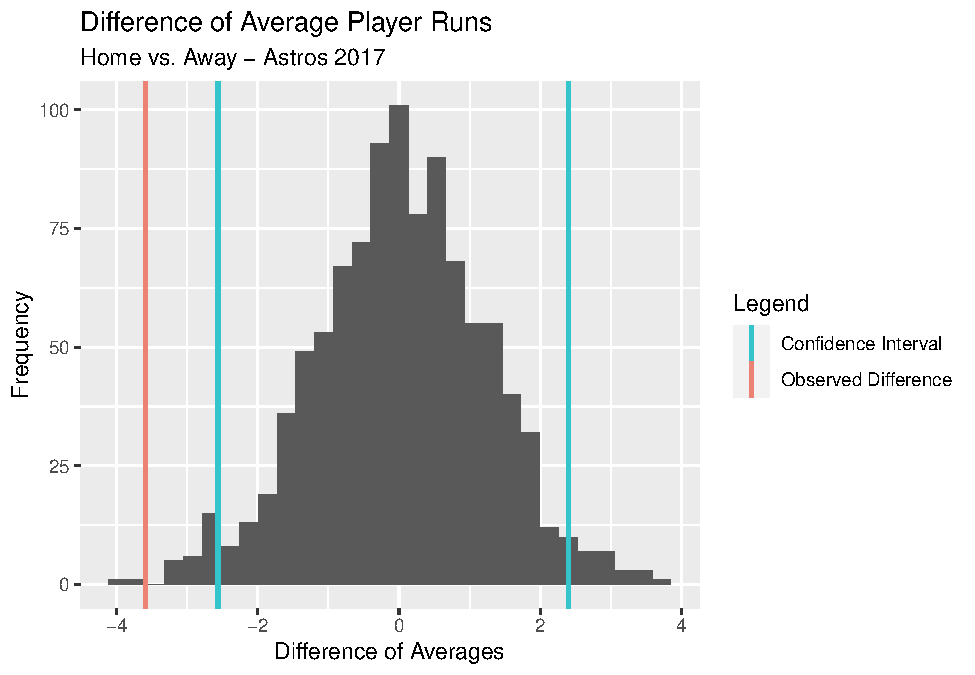
\includegraphics{Stat340_Final_files/figure-latex/mc_runs-1.pdf}

\begin{center}\rule{0.5\linewidth}{0.5pt}\end{center}

After performing a 95\% confidence interval on our data, we see that our
observed difference falls outside of the confidence interval, leading us
to reject our initial assumption. Thus, we can say with 95\% confidence
that there is statistical significance in the difference of Run means
between home and away games.

However, because Away game Runs are lower than Home game Runs, this
implies that the Atros cheating had a positive effect on their
performance.

\begin{center}\rule{0.5\linewidth}{0.5pt}\end{center}

\hypertarget{attempting-regression}{%
\subsubsection{\texorpdfstring{\emph{Attempting
Regression}}{Attempting Regression}}\label{attempting-regression}}

Next we will attempt to perform a regression to predict the percentage
of games that a team will win based on their summed statistics in Runs,
Hits, Home Runs, Runs Batted In, and split. To do this we will have to
combine a few datasets: the data we have for specific players from
baseball-reference.com and data for team statitcs (games won, lost and
played by home and away).

\begin{Shaded}
\begin{Highlighting}[]
\FunctionTok{summary}\NormalTok{(lm}\FloatTok{.2017}\NormalTok{)}
\end{Highlighting}
\end{Shaded}

\begin{verbatim}
## 
## Call:
## lm(formula = win_percent ~ R + H + HR + RBI + split, data = lm_data_2017)
## 
## Residuals:
##       Min        1Q    Median        3Q       Max 
## -0.139163 -0.049089 -0.002704  0.041373  0.151519 
## 
## Coefficients:
##               Estimate Std. Error t value Pr(>|t|)  
## (Intercept)  0.2840020  0.1583572   1.793   0.0792 .
## R            0.0044615  0.0020957   2.129   0.0384 *
## H           -0.0006206  0.0003044  -2.039   0.0470 *
## HR          -0.0003156  0.0007660  -0.412   0.6822  
## RBI         -0.0028403  0.0022090  -1.286   0.2047  
## splitHOME    0.0487977  0.0186055   2.623   0.0117 *
## ---
## Signif. codes:  0 '***' 0.001 '**' 0.01 '*' 0.05 '.' 0.1 ' ' 1
## 
## Residual standard error: 0.06507 on 48 degrees of freedom
## Multiple R-squared:  0.5357, Adjusted R-squared:  0.4874 
## F-statistic: 11.08 on 5 and 48 DF,  p-value: 3.964e-07
\end{verbatim}

From our results we can see that our regressions are very bad. None of
the p values are below .05 for both home and away games. In the future
we will really need to improve upon this model.

\hypertarget{discussion-on-progresschallenges}{%
\subsection{Discussion on
Progress/Challenges}\label{discussion-on-progresschallenges}}

\textbf{Challenges}:

\begin{itemize}
\item
  On our last project report, the results that we gathered from the data
  were not what we expected. We originally cleaned the dataset wrong and
  it affected the outcome, giving us reason to believe the Astros didn't
  cheat. After going back and changing how we read in the data, our
  graphs prove what we were originally expecting, and show initial
  evidence that they were cheating. Our original findings were very
  surprising because this cheating scandal wouldn't have been a scandal
  if it weren't for some correlation and evidence that suggest they did.
  This was a big challenge because after our last project report, we
  thought we were gonna have to go back and change our whole project.
  But now we are back on track and can continue the analysis of our
  questions.
\item
  Another challenge we faced during this project report was trying to
  figure out how to use a linear model in our analysis. We originally
  wanted to use a regression model on all of the variables in our
  dataset to predict wins and then we could see if home games (the
  supposed cheating) was a statistically significant variable. After
  initially trying this, we realized this approach was not a very
  good/strong indication of how home games helped them cheat. Then, we
  thought it would be beneficial to compare individual Astro players
  pre-season stats, to that of the regular season, and compare home and
  away. This also came with its issues though because there wasn't
  individual player data for preseason. So we moved onto our next
  thought process
\item
  From the data site Kieth gave us from the last project report, we
  found a perfect data set split up into the home and away games, but
  there were no column names for 161 variables. So we used python to
  assign column names from the reference sheet online.
\item
  In doing this, we found out how hard it is to try and piece together
  all the datasets. This method also increases the margin of error,
  which is something we can compute and analyze for the final report.
\end{itemize}

\textbf{Progress}:

\begin{itemize}
\item
  We came to the realization that some of our data cleaning from our
  last project report was skewing the results. We fixed that problem,
  re-fit the previous graphs, and re-analyzed them
\item
  We spend a tremendous amount of time reading in new data and cleaning
  it, in order to form a regression model. After forming a linear model
  to predict win\_percentage based on Runs, Hits, Runs Batted In, Home
  Runs, and Split (Home vs, Away), we found that the model sucks, like a
  lot. So we will need to adapt our model to work better in the future,
  but we did not have enough time to finish it now.
\end{itemize}

\hypertarget{next-steps}{%
\subsection{Next Steps}\label{next-steps}}

\begin{itemize}
\item
  We want to figure out why the new regression models we created were so
  bad. Before the final project is due, we will work on how to improve
  our model, and attend office hours to gain some insight as why they
  currently are the way they are. We can then plot the models to
  visually see how they are doing
\item
  We also might want to look into the performance of teams throughout
  the league at the Astros' home stadium to see if the conditions under
  which teams play at that location (called park factors) have any
  affect on performance, indicating a possible reason for the Astros
  lower performance at home.
\item
  We are also considering looking into things such as individual Astros
  players performance and test to see if there were any noticeable,
  improbable differences between years, comparing it to the change in
  performance for other teams' top performers.
\end{itemize}

\end{document}
